\documentclass[UTF8, oneside, fontset=mac]{pkuthss}
\usepackage[backend = biber, style = gb7714-2015ay,sortcites,sorting=ynt, doi=false, url=false]{biblatex}
\usepackage{ntheorem}
\usepackage{tabularx}
\usepackage{longtable,multirow,booktabs}
\usepackage{float,caption}
\usepackage{fontspec}
\usepackage{rotating}
\usepackage[perpage]{footmisc}
\theoremseparator{:}
\newtheorem{hyp}{假说}
\renewcommand{\thehyp}{H\arabic{hyp}}
% \aboverulesep=0ex
% \belowrulesep=0ex
\usepackage{arydshln}
\newif\ifblind\blindfalse
\renewcommand*{\bibfont}{\zihao{5}\linespread{1.27}\selectfont}
% \renewcommand{\thefootnote}{\@arabic\c@footnote}
\setlength{\bibitemsep}{3bp}
\newif\ifblind\blindfalse
\pkuthssinfo{
	cthesisname = {硕士学位论文}, ethesisname = {Master Thesis},
	thesiscover = {硕士学位论文},degreetype={2},
	ctitle = {极端天气冲击对家财险需求的影响——以极端降水为例},
	etitle = {The Impact of Extreme Weather Shock on Household Property Insurance Demand},
	cauthor = {董晨阳}, eauthor = {Chenyang Dong}, date = {\today},
	studentid = {2201211201}, school = {经济学院},
	cmajor = {保险学}, emajor = {Insurance},
	direction = {保险学}, mentorlines = {1},
	cmentor = {刘新立},
	ementor = {Xinli Liu},
	ckeywords = {极端天气;家财险需求;风险感知;保险市场},
	ekeywords = {Extreme Weather; Home Property Insurance Demand; risk perception; Insurance Market},
}
\addbibresource{thesis.bib}
\hypersetup{
    hidelinks,
}
\begin{document}
\frontmatter
\pagestyle{empty}
\ifblind\makeblind\else\maketitle\fi
% \clearpage
 %!TEX root = ../thesis.tex
% Copyright (c) 2008-2009 solvethis
% Copyright (c) 2010-2017,2021 Casper Ti. Vector
% All rights reserved.
%
% Redistribution and use in source and binary forms, with or without
% modification, are permitted provided that the following conditions are
% met:
%
% * Redistributions of source code must retain the above copyright notice,
%   this list of conditions and the following disclaimer.
% * Redistributions in binary form must reproduce the above copyright
%   notice, this list of conditions and the following disclaimer in the
%   documentation and/or other materials provided with the distribution.
% * Neither the name of Peking University nor the names of its contributors
%   may be used to endorse or promote products derived from this software
%   without specific prior written permission.
%
% THIS SOFTWARE IS PROVIDED BY THE COPYRIGHT HOLDERS AND CONTRIBUTORS "AS
% IS" AND ANY EXPRESS OR IMPLIED WARRANTIES, INCLUDING, BUT NOT LIMITED TO,
% THE IMPLIED WARRANTIES OF MERCHANTABILITY AND FITNESS FOR A PARTICULAR
% PURPOSE ARE DISCLAIMED. IN NO EVENT SHALL THE COPYRIGHT HOLDER OR
% CONTRIBUTORS BE LIABLE FOR ANY DIRECT, INDIRECT, INCIDENTAL, SPECIAL,
% EXEMPLARY, OR CONSEQUENTIAL DAMAGES (INCLUDING, BUT NOT LIMITED TO,
% PROCUREMENT OF SUBSTITUTE GOODS OR SERVICES; LOSS OF USE, DATA, OR
% PROFITS; OR BUSINESS INTERRUPTION) HOWEVER CAUSED AND ON ANY THEORY OF
% LIABILITY, WHETHER IN CONTRACT, STRICT LIABILITY, OR TORT (INCLUDING
% NEGLIGENCE OR OTHERWISE) ARISING IN ANY WAY OUT OF THE USE OF THIS
% SOFTWARE, EVEN IF ADVISED OF THE POSSIBILITY OF SUCH DAMAGE.

% 此处不用 \specialchap,因为学校要求目录不包括其自己及其之前的内容。
\chapter*{版权声明}
% 综合学校的书面要求及 Word 模版来看,版权声明页不用加页眉、页脚。
\thispagestyle{empty}

任何收存和保管本论文各种版本的单位和个人,
未经本论文作者同意,不得将本论文转借他人,
亦不得随意复制、抄录、拍照或以任何方式传播。
否则,引起有碍作者著作权之问题,将可能承担法律责任。

% 若须排版二维码,请将二维码图片重命名为“barcode”,
% 转为合适的图片格式,并放在当前目录下,然后去掉下面 2 行的注释。
\vfill\noindent

\includegraphics[height = 5em]{img/barcode.png}

% vim:ts=4:sw=4

\clearpage
\pagestyle{plain}
\setcounter{page}{0}
\pagenumbering{Roman}
%!TEX root = ../thesis.tex
\begin{cabstract}
    随着全球气候变化的加剧,极端天气事件对人类社会和经济活动的影响日益凸显。本研究基于极端降水冲击的准自然实验,以某公司家财险数据,采用差分分析方法探究极端天气冲击对家财险购买的影响。结果表明,极端天气冲击后,家财险的保额整体上显著提高7\%,20-50公里的近灾区相较于未受影响的地区保额进一步提升9\%,但是冲击20公里内的灾区由于受获得性启发机制及赔付的逆选择影响,保额下降了30\%,且回归结果通过了稳健性检验。进一步的分析揭示极端天气过往经历的适应性预期不足、巨灾导致的风险敏感度提升、保险标的的高价值以及城乡风险感知的差异都会对极端降水冲击带来的家财险需求有正向提升作用。本文的研究为极端降雨与家财险购买的因果关系提供了经验证据,在微观层面理解气候变化对个体风险决策的冲击提供了新的视角。
\end{cabstract}
\begin{eabstract}
    With the intensification of global climate change, the impact of extreme weather events on human social and economic activities has become increasingly prominent. Based on the quasi-natural experiment of extreme precipitation shock, this study uses the differential analysis method to explore the impact of extreme weather shock on the purchase of family property insurance based on the property insurance data of a company. The results show that after the extreme weather shock, the insurance amount of family property insurance is significantly increased by 7\%, and the insurance amount of the near disaster area of 20-50 km is further increased by 9\% compared with the unaffected areas. however, due to the influence of the adverse selection mechanism of acquisition inspiration and compensation, the insurance amount of the disaster area within 20 km decreased by 30\%, and the regression results passed the robustness test. Further analysis reveals that the lack of adaptive expectations of extreme weather past experience, the increase of risk sensitivity caused by catastrophes, the high value of the subject matter of insurance and the difference in risk perception between urban and rural areas will have a positive effect on the demand for family property insurance caused by extreme precipitation shocks. The study of this paper provides empirical evidence for the causal relationship between extreme rainfall and family property insurance purchase, and provides a new perspective to understand the impact of climate change on individual risk decision-making at the micro level.
\end{eabstract}

\tableofcontents
\mainmatter
%!root = ../main.tex
% 极端气候定义、风险偏好=>风险厌恶程度、家财险定义
\chapter{引言}
\section{研究背景}

% 背景、政策、数据
2023年10月24日,我国政府宣布增发2023年国债1万亿元,集中用于灾后恢复重建和提升国家防灾减灾能力。这一决策表明政府对气候变化带来的灾害风险的高度关注,也突显了防灾减灾工作的紧迫性。在现代社会,气候变化已经成为一个备受瞩目的全球性问题。
近年来,极端天气事件也层出不穷。据统计,全球范围内的极端天气事件频率和强度都在不断增加。这些极端天气事件包括暴雨、洪水、干旱、飓风等,给人们的生活和财产带来了巨大的风险和损失。极端天气频繁发生给人们造成物质上的创伤同时,也对人们的风险偏好有着潜移默化的影响,例如位于台风路径上的企业更偏好持有现金\citep{杨娜娜2019自然灾害与企业现金持有}。极端天气冲击对人们风险偏好是否会产生影响以及产生何种影响是一个值得研究的课题,能帮助我们提前做好风险管理措施,而不是总是亡羊补牢。
% 分散风险是重要课题
\begin{table}[H]
    \centering
    \caption{2023年我国部分极端天气事件}
    \begin{tabular}{@{}ccc@{}}
        \toprule
        \textbf{日期} & \textbf{事件类型} & \textbf{影响地区}&\textbf{直接经济损失金额} \\
        \midrule
        1月1日至6月9日   & 严重冬春连旱        & 云南            \\
        4月至5月       & 高温热浪          & 华北、黄淮地区       \\
        5月下旬至6月上旬   & 大范围降水         & 河南、陕西     \\
        7月28日       & 台风“杜苏芮”       & 福建晋江沿海        \\
        7月29日至8月1日  & 极端暴雨          & 京津冀地区         \\
        8月初         & 强降雨           & 东北地区          \\
        9月3日        & 台风“海葵”登陆      & 台湾省台东市        \\
        12月14日至17日  & 全国型寒潮         & 全国60\%以上国土面积  \\
        2023年全年     & 全国平均气温偏高      & 全国大部地区        \\
        2023年全年    & 沙尘天气过程增多      & 全国            \\
        2023年全年       & 极端降水          & 广西北海市     \\
        2023年全年       & 强对流天气         & 全国\\
        \bottomrule
    \end{tabular}
    数据来源:国家气象局
\end{table}

随着极端气候事件的频繁发生,人们对自身及财产的安全日益关切。在灾害面前,家庭往往是首当其冲的受害者。但与企业相比,个人家庭对这些潜在风险的反应可能更为复杂。家庭是否会通过购买家财险来缓解财产损失,以及他们在灾害发生后是否更加倾向于购买保险,这些问题有许多影响因素,具有较强的实证研究价值。

然而,极端天气下人们对自身及财产安全的关切是否能够持续转化为对保险的需求,尤其是在家庭层面,却是一个相对较少被深入研究的领域。过去的国内研究主要关注气候变化对企业财产险或健康险的影响,比如雾霾天导致大量健康险投保之后又退保等,但是对于家庭财产保险的定量研究却相对较少。本研究的选题来源于对这一领域的关注,力图深入了解极端天气极端冲击对风险偏好的影响,填补现有研究的空白。

作为风险管理的手段之一,我国的家财险始于1980年,是当时中国人保重点推广的基础险种之一。在1980年,全国范围内有34200户家庭购买了中国人保的家财险,承保金额为5232万元,保费仅为7万元,仅占国内产险保费总额的0.02\%。到了1989年,全国家财险(包括储蓄性两全险)的投保户数增至7691万户,承保金额达1974亿元,保费收入为3.2亿元,占产险保费总额的4.4\%。可以说,我国财产保险的早期发展同时也是家庭财产保险演进的历史\citep{黄英君2008论我国产险公司分散性业务营销模式的创新},塑造了国人对财产险最早的认知。
2023年10月24日,我国政府宣布增发2023年国债1万亿元,集中用于灾后恢复重建和提升国家防灾减灾能力。这一决策表明政府对气候变化带来的灾害风险的高度关注,也突显了防灾减灾工作的紧迫性。在现代社会,气候变化已经成为一个备受瞩目的全球性问题。随着极端气候事件的频繁发生,人们对自身及财产的安全日益关切。在灾害面前,家庭往往是首当其冲的受害者。但与企业相比,个人家庭对这些潜在风险的反应可能更为复杂。家庭是否会通过购买家财险来缓解财产损失,以及他们在灾害发生后是否更加倾向于购买保险,这些问题有许多影响因素,具有较强的实证研究价值。

我国的家财险始于1980年,是当时中国人保重点推广的基础险种之一。在1980年,全国范围内有34200户家庭购买了中国人保的家财险,承保金额为5232万元,保费仅为7万元,仅占国内产险保费总额的0.02\%。到了1989年,全国家财险(包括储蓄性两全险)的投保户数增至76,910,000户,承保金额达1974亿元,保费收入为3.2亿元,占产险保费总额的4.4\%。可以说,我国财产保险的早期发展同时也是家庭财产保险演进的历史\citep{黄英君2008论我国产险公司分散性业务营销模式的创新},塑造了国人对财产险最早的认知。自那时起我国家财险保费收入持续提升,市场蓬勃发展,2022年家财险以67.22\%的增长率成为了保费增速最快的产险险种,保费达到164亿,但家财险2022年末在行业保费规模中占比仅1.1\%。

在此背景下,我们将通过深入研究极端天气对家财险需求的影响,探索个人家庭在面对气候变化时的风险管理行为,为保险业和政策制定提供更为全面的了解。本研究的意义不仅仅停留在学术探究层面,更涉及到实际社会和经济层面的多个方面:

首先,通过深入研究极端天气对家财险需求的影响,我们能够为保险公司提供更为精准的市场预测。这对于保险公司的产品开发、定价和风险管理具有重要指导意义。预测气候事件可能引发的家财险需求波动,可以帮助保险公司制定更灵活的营销策略,及时调整产品组合,提高市场适应性。

其次,研究家财险需求的变化还能够提供社会科学领域对于人类行为和决策的深刻洞察。了解在灾害面前个体的风险认知和行为模式,有助于拓展对人类在危机时刻的心理和社会反应的认知。这对于制定个体和社会层面的应对策略,以及心理健康服务的提供都具有积极的实践意义。

最后,从可持续发展的角度来看,本研究有助于引导人们更加理性和科学地对待气候变化风险。通过了解保险在气候变化应对中的作用,可以提高社会对于个体责任和社会共担责任的认识。这有助于形塑一种更加可持续、共同应对气候挑战的社会文化氛围。

\section{研究方法:研究极端降水冲击如何影响家财险需求}
本文对于极端天气冲击风险偏好的研究方法是通过实证分析极端降水对家财险需求的影响。极端天气冲击根据ETCCDI\citep{alexander2006global}定义可以分为两大类:极端降水和极端温度。本文选取极端降水作为研究对象,通过实证分析极端降水对家庭财产保险需求的影响,以此探究极端天气事件对家庭风险偏好的影响。

本文的分析方法包括回归分析和差分分析。首先,本文基于某保险公司保单数据以及气象站数据整理出一个家庭财产保险标的与天气灾害的联合分布数据集,包括家庭财产保险标的的保额、保费、地理位置等信息,以及该距离标的相匹配的时空上最近和较近的气象站极端降水事件的发生时间、地点等信息。然后,我们将通过描述性统计的方法,对家庭财产保险数据集的保额、保费、地理分布等特征进行描述性统计,以了解家庭财产保险的基本情况。再次,我们将通过回归分析的方法,探究极端天气事件对家庭财产保险需求的影响。我们将构建多元线性回归模型,控制其他因素的影响,研究极端天气事件对家庭财产保险保额的影响。最后,我们将通过差分分析的方法,进一步探究极端天气事件对家庭财产保险需求的影响,我们将构建双重差分模型,研究极端天气事件对家庭财产保险保额的影响,并对灾区和非灾区的影响进行比较,探究不同地区家庭行为的差异和背后潜在的原因。

本文的结构安排如下:第\ref{chap:2}章是文献综述与研究假说。我们将梳理关于气候变化对保险需求影响的研究,探讨风险偏好的相关理论及其影响因素,分析自然灾害如何影响个人和企业的风险偏好,以及这些变化如何反映在保险购买行为上。在文献综述的基础上,我们将提出本研究的三个主要假设。这些假设的提出基于现有文献的不足和本研究的独特视角,旨在填补关于家庭财产保险需求对极端天气事件反应的研究空白。

第\ref{chap:3}章研究设计将详细介绍本研究所采用的方法论框架、数据来源及处理方式、以及模型设定和变量定义。首先,我们将界定极端天气事件的范围,并根据ETCCDI标准选取极端降水作为研究重点。接着,我们将描述样本选择的过程,包括数据的时间和空间范围,以及数据清理的具体步骤。最后,我们将详细阐述所采用的计量经济模型,包括基础的回归分析和双重差分(DID)方法,并解释模型中各变量的经济含义及其预期的作用。

第\ref{chap:4}章实证分析将展示对家财险需求影响的实证结果。本章将首先提供描述性统计数据,以揭示样本的基本特征。随后,我们将报告回归分析的结果,包括基础回归和DID回归模型的估计结果,以及对模型稳健性的检验。此外,我们还将探讨极端天气事件对保险赔付和续约行为的影响,通过Logit回归分析来深入理解居民和保险公司在灾害后的行为变化。

第\ref{chap:4.1}章主要是扩展问题的实证结果,主要讨论地理位置和保单购买时间等不同时,极端天气对家庭购买家财险的横截面差异,进一步加强本文基本问题的逻辑性。

第\ref{chap:5}章将总结本研究的主要发现,并讨论其对保险业和政策制定的潜在影响。我们将回顾研究假设的验证情况,探讨极端天气事件对家庭风险偏好和保险需求的影响机制,并提出未来研究的可能方向。同时,我们也将讨论本研究的局限性,并就如何提高家庭财产保险市场的适应性和效率提出建议。

\chapter{文献综述与研究假说}\label{chap:2}
\section{文献综述}

本文主要从两个角度梳理国内外相关文献:一是风险偏好的影响因素,二是极端天气变化对不同保险需求的影响。

\subsection{自然灾害与风险偏好}

自然灾害会对企业风险偏好产生影响,例如位于台风路径上的企业更偏好持有现金\citep{杨娜娜2019自然灾害与企业现金持有}或调整债务结构\citep{shao2024typhoons}以应对风险。有研究基于可得性启发式理论\citep{0Do},指出尽管飓风并未实质性地改变未来飓风发生的概率,管理者仍倾向于通过增加现金储备来应对这种突如其来的风险,但不同距离灾区公司的反映是不同的,灾区公司受到了飓风的直接影响,因此它们的现金持有量出现了显著的下降,现金水平平均下降了约1400万美元。邻近区域公司虽然未直接受到飓风的影响,但由于地理位置接近灾区,飓风事件对它们的管理者来说是显著的,现金持有量平均增加了1.1\%。这种增加是暂时的,随着时间的推移,现金持有量逐渐回到了飓风前的水平。其他地区距离飓风灾区较远,飓风事件对它们的显著性较低。该研究的发现支持了显著性理论的观点,即决策者的注意力容易被显著事件所吸引,从而在风险评估中给予这些事件过高的权重。但随着台风发生次数的增加,管理层的过度反应现象有所减弱,这表明经验的积累可能有助于提高企业对自然灾害的反应效率。

而家庭侧风险偏好影响因素方面,大多数研究主要从个体的角度出发,例如以收入\citep{石双2018收入与风险偏好}、资产总额\citep{卢亚娟殷君瑶2021户主风险态度对家庭金融资产配置的影响研究}、年龄\citep{王晶2021年龄结构}、健康状况\citep{雷晓燕2010中国家庭的资产组合选择}、教育程度\citep{梁立俊2018受教育程度与主客观风险偏好}、职业\citep{赵颖2017中国劳动者的风险偏好与职业选择}、性别\citep{徐小华2019女性劳动参与会影响家庭资产配置风险偏好吗}等为主要研究对象。例如有研究利用CHFS数据,采用Probit、Tobit模型及倾向得分匹配法(PSM),从整体和城乡两个维度出发,深入研究了户主的风险态度对家庭金融资产配置的影响\citep{卢亚娟殷君瑶2021户主风险态度对家庭金融资产配置的影响研究}。研究发现,风险偏好的家庭表现出更高的金融资产参与率和资产占比,且其对金融市场,特别是风险市场的参与行为更为积极。进一步的分析揭示,风险偏好的家庭在风险性金融资产投资上占据主导地位,尤其是在股票方面表现最为显著;相反,家庭越厌恶风险,则其对股票的投资越低。在考察城乡差异时,研究发现户主风险态度对于家庭金融资产选择产生不同影响,尤其是在城镇家庭的风险性金融资产投资方面,风险态度的影响更为显著。

外生事件冲击方面,有研究以中国2003-2005年发生的4次地震为案例,利用国家统计局城镇住户调查数据,通过双重差分法的研究方法,探讨地震对城镇家庭风险偏好的影响及其背后的机制\citep{章元0地震冲击对风险偏好的影响}。地震显著提高了城镇家庭的风险厌恶程度。尤其是距离震中越近的家庭,在地震发生后,购买彩票的概率和支出下降越为显著。这一结果揭示了地震引起的风险预期上升和负向情绪冲击是重要的机制。进一步分析显示,距离震中越近的家庭,其震后非储蓄性保险支出以及用于缓解负向情绪的消费支出上升越多。这意味着地震对家庭风险偏好的影响,不仅体现在经济决策上,还体现在对非储蓄性保险和消费行为的调整上。

风险偏好可以通过商业保险购买决策体现,即风险偏好与商业保险购买之间存在正向关系\citep{宋章良2021我国中老年家庭风险偏好对商业保险购买行为的影响研究},但这一现象的主要原因在于反向因果关系,即高风险偏好的家庭更倾向于购买投资型保险而非保障型保险,与此同时该群体的人均收入较高。也有观点认为购买商业保险也会改变家庭风险偏好\citep{孙武军2023商业健康保险的配置能够改变家庭的风险偏好吗},其以2017年中国家庭金融调查(CHFS)数据为基础,将家庭风险偏好划分为主观和客观两个方面,旨在深入探讨商业健康保险配置对我国居民家庭主客观风险偏好的实证影响。通过采用有序Probit模型进行估计,研究在控制了多个关键因素(包括人口统计特征、健康状况、家庭经济状况以及社会保险持有情况)的基础上,如何处理可能存在的内生性问题。研究的主要发现表明,家庭配置商业健康保险能够显著提高家庭的主客观风险偏好。此外,通过对异质性分析的深入研究,发现这种正面影响在低收入家庭中尤为显著,而在高收入家庭中则作用较为微弱。

总体而言,自然灾害对风险偏好影响的研究在企业侧研究更为充分,而对家庭侧风险偏好的研究主要集中在风险偏好如何影响家庭金融资产配置、消费行为等方面,对极端天气事件如何塑造家庭风险偏好的研究相对较少。本文将探究极端天气冲击对家庭风险偏好的影响,以探究气候变化如何塑造人类行为。

\subsection{极端天气冲击对不同种类保险需求的影响}

一般认为极端天气是指气象要素的极端值,包括极端温度、极端降水、极端风速、极端湿度、极端干旱等\citep{傅良2022ECMWF,吴大明2021近年来全球极端天气气候事件情况及影响分析}。极端天气事件是指在一定时间和空间范围内,气象要素的极端值或极端变化,如暴雨、洪水、干旱、飓风、暴风雪等。得益于广泛的数据积累,有研究表明极端气温和降水近几十年来的强度和频率发生了变化\citep{ummenhofer2017extreme}。极端天气事件的发生频率和强度都在不断增加,给人们的生活和财产带来了巨大的风险和损失。极端天气事件对保险需求的影响是一个备受关注的课题,国内外学者已经开展了大量的研究。关于极端天气冲击对保险需求的影响,有关研究主要集中在寿险、健康险和农险上,对家财险的研究较少。

健康险方面,空气污染水平对健康险的购买或退保的决策产生的显著影响\citep{2018Something},每日空气污染水平每增加一个标准差,当天销售的保险合同数量增加了7.2\%。而在考虑购买后的条件下,即在冷静期内,相对于订单日期水平,每日空气污染水平每减少一个标准差,退保概率增加了4.0\%,研究还探讨了多种可能的机制,发现了对投射偏差和显著性的最有力支持。也有研究旨在探究空气污染对中国居民商业健康保险需求的影响大小\citep{赵强2021空气污染对商业健康保险需求的影响},利用2011年至2016年秦岭淮河地区84个地级市的宏观数据,采用模糊断点回归设计和中国北方集中供暖政策的准自然实验方法,旨在深入了解空气污染对中国居民商业健康保险需求的影响。结果显示,空气污染对商业健康险需求存在显著的正向影响,特别是PM2.5污染物的排放浓度每提升1\%,商业健康保险密度提高1.098\%。即便在考虑六种不同污染物指标的情况下,估计结果仍然趋近一致。值得关注的是,从2013年开始,我国经历了大范围持续的雾霾天气,伴随着新闻媒体报道频率的增加。这导致居民对空气污染的敏感度和重视度逐渐提高,进而反映在对商业健康保险的购买上。

而对于极端天气冲击对健康险需求的影响机制,研究观点主要集中在极端天气冲击影响的个人风险偏好。例如有研究认为空气污染提升了个人的风险感知,进而引起健康保险需求增加\citep{宋平凡2022空气污染}。其基于2006—2016年中国283个地级以上城市的数据,系统考察了空气污染对健康保险需求的实证影响,采用百度指数作为风险感知的代理变量,并运用中介效应模型验证了空气污染对健康保险需求的影响机制。结果显示,通过百度指数体现的风险感知效应是空气污染引起健康保险需求增加的重要途径,并且工具变量中介效应模型的实证结果进一步支持了这一结论。还有研究认为气候变化增加了居民对气候风险和健康的关注\cite{zhong2022exposure},其利用CHARLS的数据集研究了异常高温对居民购买商业健康保险的影响,发现,随着异常温度每升高1°F,人们购买商业健康保险的概率增加了6\%。此外,性别和地域因素也显得尤为重要,研究表明异常高温对女性、南方居民和东部居民的商业健康保险需求产生更为显著的影响。其认为异常高温对商业健康保险需求的影响机制包括:增加了居民对气候风险的关注,使其更倾向于购买健康保险以规避潜在的健康风险;异常高温对健康的实质性影响也使居民更加关注自身的医疗保障需求。

极端天气冲击对寿险需求也有一定的的影响。例如对于欧盟成员国,有研究采用面板模型,研究保费金额和温室气体排放的关系\citep{melnychenko2021influence},根据其实证研究的结果,每千吨温室气体排放的增加导致寿险保费金额增加17万欧元,具有显著性。而影响机制方面,有观点研究2013年德国洪水对个人的冲击\citep{avdeenko2021impact},认为这种变化是风险厌恶选择导致高风险地区人寿保险需求的增加,通过幸福感的变化来介导,从而解释了风险偏好的改变。

财险方面,天气灾害对汽车出险有一定的影响,有关研究发现近年来天气灾害致汽车出险的数量明显增加\citep{张翠华2020天气灾害致车险理赔的风险分析},其研究数据集为河北省2004-2018年天气灾害致车险理赔事故,研究发现主导汽车出险的天气灾害主要包括暴雨、涉水、冰雹和暴风,在不同地区出险数量存在明显的差异。

其他财险险种方面的研究主要集中在农业保险领域,例如研究极端天气冲击对农险需求的影响\citep{胡新艳2021气候变化},通过地级市气候数据和农户微观数据进行匹配,进行了实证分析。研究发现,气候变化在显著促进农户农业保险购买行为方面发挥了关键作用,但在不同生产目的的农户中存在异质性影响。具体而言,当农户的经营目标从满足自家消费转向为追求市场利润时,其购买农业保险的需求更为强烈。进一步分析表明,气候变化导致的两类农业风险对农户购买农业保险的中介作用存在差异。土壤退化风险由于具有渐进性,农户能够在农业生产之前通过调整生产要素供给来降低风险损失,因此对农业保险的需求较为低迷。相反,病虫害风险属于突发性风险,农户难以通过事前风险防控来分散风险,从而强化了其对农业保险的需求。

此外还有研究极端天气冲击对信贷保证保险需求的影响的研究\citep{张钦2017高寒生态脆弱区农户对气候变化的适应需求},以甘南高原为研究区域,通过对500份农户调查问卷的分析,揭示了气候变化对不同区域和生计方式的农户产生的影响及其适应需求。研究发现,农户在适应极端天气冲击的过程中,对基础设施的需求最为迫切,紧随其后的是对信息和生产技术的需求。进一步分析表明,不同区域和生计方式的农户对适应极端天气冲击的需求存在显著差异。在区域方面,纯牧区和农区农户对基础设施的需求最为强烈,而半农半牧区农户更加关注信息的获取。而在生计方式上,纯农户对信贷保险的需求最为迫切,而一兼户和二兼户则更加倚重基础设施的提升。进一步的分析揭示了影响不同适应需求的关键因素,如自然资本和物质资本对生产技术需求的影响,自然资本和人力资本对信息需求的影响,人力资本和金融资本对基础设施需求的影响,以及多个因素共同影响信贷保险需求。

总体而言,国内外关于极端天气冲击对保险需求的影响研究主要集中在健康险、寿险和农险领域,而对于家庭财产保险的研究相对较少。本文将从家庭财产保险的角度出发,深入探究极端天气冲击对家庭财产保险需求的影响机制,填补现有研究的空白。

\section{研究贡献与研究假设}
本文的研究贡献主要体现在以下几个方面:

第一,本文填补了国内关于极端天气事件对家庭财产保险需求冲击的研究空白,为我国家庭财产保险需求的研究提供了新的视角。已有的极端天气研究大多以企业 \citep{0Do}或是健康险\citep{赵强2021空气污染对商业健康保险需求的影响}、农险\citep{胡新艳2021气候变化}为主,对家庭的关注则较少。

第二,本文通过海量数据的实证分析,深入探究了极端天气事件对家庭财产保险需求的影响机制,探究了灾区和非灾区家庭财产保险需求的差异,为政府和监管机构制定相关政策提供了参考。

最后,本文通过实证研究,为社会科学领域对于人类行为和决策的深刻洞察提供了新的案例,为其他学科的研究提供了新的视角。

本研究旨在探讨极端天气事件如何影响家财险需求,进而研究人们的风险偏好在极端天气事件影响下的变化。本文将从时间维度和空间维度两个角度出发,提出以下三个研究假设:

首先,在时间维度上,极端天气事件的发生会直接影响居民的风险感知,使其对极端天气事件的风险有了更为直观的认识,居民的风险偏好可能会发生变化,从而影响其对家财险的需求。类似于台风路径下的企业持有现金\citep{0Do}和雾霾增加健康险购买\citep{赵强2021空气污染对商业健康保险需求的影响},根据可得性启发式理论\citep{tversky1973availability},人们倾向于依赖最容易回忆起的信息来做出判断。极端天气事件因其罕见和强烈的影响,往往会在居民心中留下深刻印象。这种直观的记忆使得居民在评估风险时更可能高估极端天气事件的发生概率,从而影响他们的风险感知。并且当人们在面对持续的风险时,可能会发展出适应性的行为和心理机制\citep{gigerenzer2011heuristic}。在经历了极端天气事件后,居民可能会调整自己的生活方式和消费习惯,以适应这种风险。这种适应性行为可能包括购买保险,以减少未来可能的经济损失。因此本文认为极端天气事件发生后,居民由于直接感知到面临极端天气事件的威胁,其居民风险感知将显著提高,从而导致他们的风险偏好增加,表现为对家财险需求的增加。基于以上分析,本文提出如下研究假说:

\begin{hyp}[H\ref{hyp:1}] \label{hyp:1}
    发生极端天气事件后,居民风险感知增加,风险偏好显著提升购买家财险的需求增加。
\end{hyp}

其次,在空间维度上,临近灾区的地区虽然未直接受灾,但由于地理位置接近灾区,极端天气事件对其风险偏好的影响可能显著\citep{0Do},导致家财险需求显著增加。临近灾区的地区可能会经历风险传递效应,即直接灾害的影响通过心理、经济和社会网络传递给周边地区。这种效应可能导致居民对潜在灾害的担忧增加,从而提高了他们对保险产品的需求。并且目睹或听闻邻近地区的灾害事件,可能会改变居民的心理预期,使他们更加关注自身的安全和财产保护。这种心理上的变化可能会导致居民采取更为保守的风险管理策略,比如购买家财险等。基于以上分析,本文提出如下研究假说:

\begin{hyp}[H\ref{hyp:3}] \label{hyp:3}
    发生极端天气事件后,临近的地区对风险厌恶增加显著,家财险需求显著增加。
\end{hyp}

最后,在空间维度上,灾区虽然直接受灾,但由于极端天气造成的直接损失可能相对有限,直接受灾或是频繁受灾的地区风险偏好可能并未显著增加\citep{shao2024typhoons},即家财险需求并未显著增加。具体而言,受灾地区的居民可能对极端天气事件有更深刻的认识和更高的风险感知。但一方面,这并不意味着他们的风险偏好会随之增加,居民可能通过其他方式来管理和降低风险,如加强房屋建设标准、改善基础设施等,从而减少了对保险的需求。另一方面,受灾地区的居民可能会发现,即使购买了家财险,也无法完全避免极端天气事件带来的损失,从而对家财险的效用产生怀疑,进而降低了对家财险的需求。基于以上分析,本文提出如下研究假说:

\begin{hyp}[H\ref{hyp:2}] \label{hyp:2}
    发生极端天气事件后,直接受到极端天气事件冲击的地区对风险偏好影响有限,家财险需求并未显著增加。
\end{hyp}

%! TEX root = ../main.tex
\chapter{研究设计}\label{chap:3}
\section{样本选择与数据来源}
\subsection{极端天气样本与数据}\label{sec:def}

气候代表了一个地区在一定时间跨度内所经历的天气状况的总体特征,揭示了一个地区的基本气象冷热、干湿特性,故而温度和降水是构成某一地区气候特征的两个最根本的气象要素\citep{alexander2006global}。在气候变化的大背景下,异常气候以及极端天气事件发生的可能性增加\citep{aigner2023summary,donat2017addendum},这其中极端强降水愈发频繁\citep{trenberth2010relationships}。在我国,极端天气事件如洪涝、干旱、台风、暴雪等自然灾害\citep{尹红2019基于},往往与极端强降水事件密切相关,给国家和人民带来了巨大的损失。因此,本文选取将极端降水作为极端天气事件的代表来,数据来源于国家气候中心,时间范围为1954年至2019年。

对于极端降雨强度的定义,国家标准 GB/T 33680-2017《暴雨灾害等级》中将日降水量超过 50mm 定义为暴雨,超过 250mm 定义为特大暴雨。然而,由于不同地区在气候特征和降水模式上存在显著差异,单一的数值标准可能无法全面反映极端降水事件的影响。参考国际气候变化检测和指数专家组(ETCCDI)采用分位数来定义极端天气的方法,将日降水量超过95th或99th百分位数的情况定义为极端降水\footnote{资料来源:UVIC,\url{https://etccdi.pacificclimate.org/list_27_indices.shtml}}。这种方法能够更好地适应不同地区的降水特征\citep{karl1999clivar},因此本文选择将极端降水天气定义为20年一遇的降水天气。
\begin{figure}[H]
    \begin{minipage}{0.48\linewidth}
        \centering
        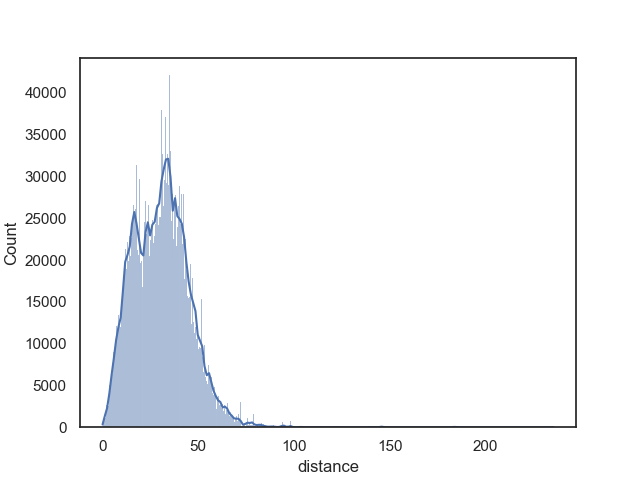
\includegraphics[width=\textwidth]{lib/img/distance.png}
        \caption{保险标与最临近气象站距离分布(千米)}
        \label{fig:distance}
    \end{minipage}
    \begin{minipage}{0.48\linewidth}
        \centering
        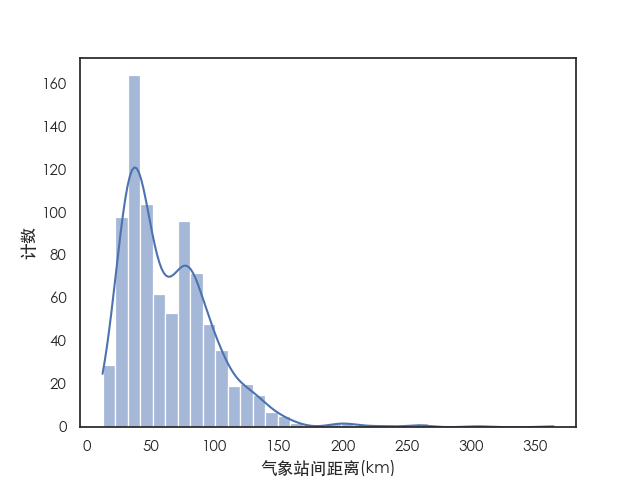
\includegraphics[width=\textwidth]{lib/img/locations_distance.png}
        \caption{气象站间距的地理位置分布(千米)}
        \label{fig:locations}
    \end{minipage}
\end{figure}

而关于极端降雨受灾范围的界定,结合降水数据和保单数据(见\ref{sec:data}),考虑到绝大多数保险标的与距离最近的气象站之间距离大多在50公里以内,平均距离不足30公里,如图\ref{fig:distance},因此本文将距离监测到极端降水的气象站20公里内的区域定义为灾区。而考虑到我国气象站分布间距基本在100公里以内,如图\ref{fig:locations},因此取气象站所覆盖的受灾半径最多为50公里,定义距离监测到极端降水的气象站20-50公里内的区域为近灾区,50公里以上的区域为远灾区。

气象站地理位置分布如图\ref{fig:location}-图\ref{fig:end}所示。

\begin{figure}[H]
    \centering
    \begin{minipage}{0.48\linewidth}
        \includegraphics[width=\textwidth, trim=200 0 200 0]{lib/img/locations.png}
        \caption{所有气象站的地理位置分布}
        \label{fig:location}
    \end{minipage}
    \begin{minipage}{0.48\linewidth}
        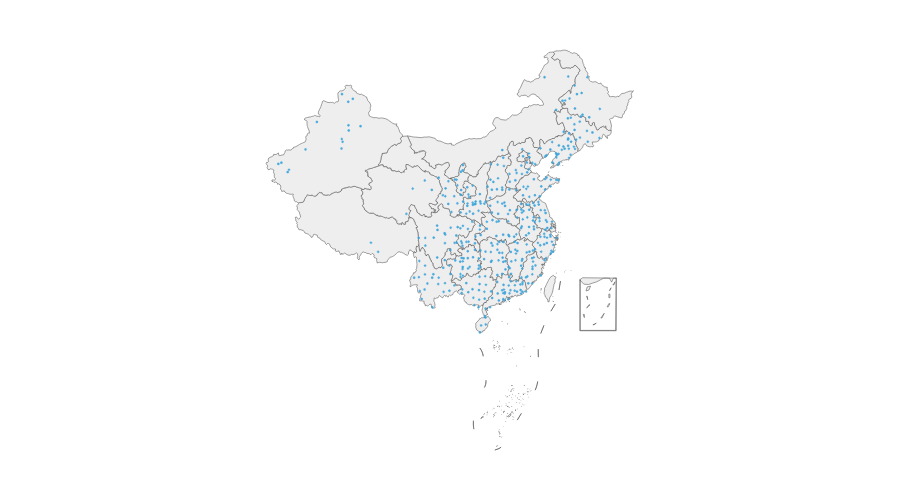
\includegraphics[width=\textwidth, trim=200 0 200 0]{lib/img/near.png}
        \caption{划分为灾区气象站的地理位置分布}
    \end{minipage}
\end{figure}
\begin{figure}[H]
    \begin{minipage}{0.48\linewidth}
        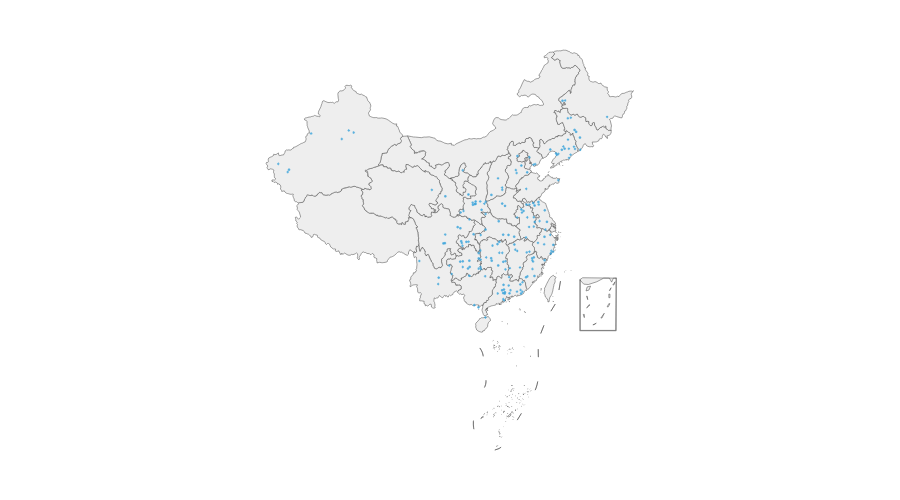
\includegraphics[width=\textwidth, trim=200 0 200 0]{lib/img/middle.png}
        \caption{划分为近灾区气象站的地理位置分布}
    \end{minipage}
    \begin{minipage}{0.48\linewidth}
        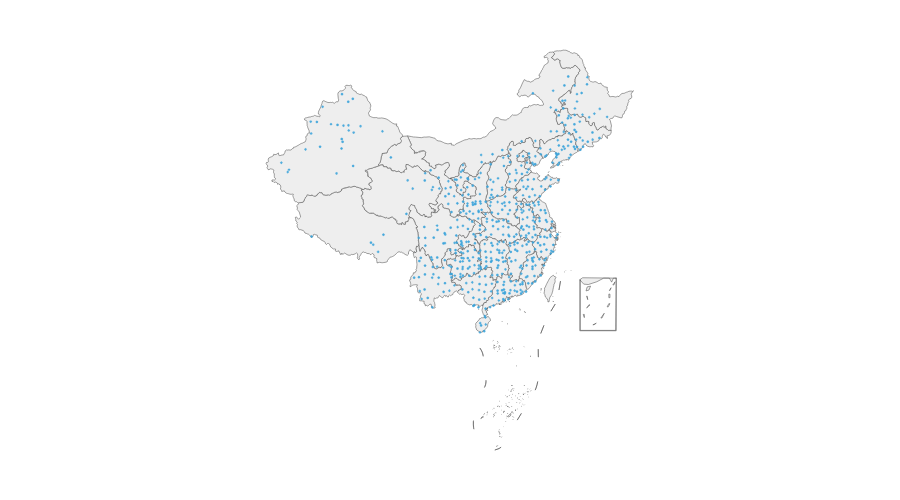
\includegraphics[width=\textwidth, trim=200 0 200 0]{lib/img/far.png}
        \caption{划分为非灾区气象站的地理位置分布}
        \label{fig:end}
    \end{minipage}
\end{figure}
\subsection{保险标的样本与数据}\label{sec:data}
本文以某财产保险公司1995年1月1日至2015年12月31日全国家财险承保理赔数据作为研究样本。

为了确保气象数据与标的样本之间的相关性,对样本基于距离进行了筛选,只选择了那些距离最近的气象站20公里以内的标的样本,然后再进行灾区、近灾区和非灾区划分进行分析。最终得到约了70万条可用于回归分析的数据。为降低异常值,影响本文对所有连续变量进行了1\%缩尾处理。

\section{模型设定与变量选取}
\subsection{变量定义}
为了更清晰地评估极端天气事件的影响,本文纳入一系列控制变量。这些变量包括:

\begin{enumerate}
    \item 是否历史投保:该保险标的是续保还是首次投保,续保的保险标的可能更倾向于保额覆盖更高的保险
    \item 保险财产的购置价:反映了家庭财产的价值,通常财产价值越高,对风险的担心也越大,保险需求也越大。
    % \item 建筑面积:建筑面积越大,需要更高的保险保额来覆盖潜在的风险。
    \item GDP增速:反应当地经济增长率,经济增长会促进保险购买。
    \item 保险深度:反映了当地保险市场的发展程度,保险市场发展程度越高,家庭购买保险的可能性也越大。
\end{enumerate}

被解释变量与控制变量含义如表\ref{tab:var}所示。
\begin{table}[H]
    \caption{变量定义表}\label{tab:var}
    \centering
    \begin{tabular}{@{}cccc@{}}
        \toprule
        变量类别                    & 变量名称         & 变量定义    & 变量解释                \\ \midrule
        被解释变量                   & Coverage     & 保额      & 保险金额                \\ \midrule
        \multirow{3}{*}{主要解释变量} & Disaster     & 灾区      & 是否处于极端降水监测点20公里内    \\ \cmidrule(l){2-4}
                                & Neighbor     & 近灾区     & 是否处于极端降水监测点20-50公里内 \\ \cmidrule(l){2-4}
                                & Post         & 降水发生时间  & 是否在极端降水发生后投保        \\
        \midrule
        \multirow{3}{*}{控制变量}   & Prem\_before & 历史投保    & 保险标的是否有投保记录         \\ \cmidrule(l){2-4}
                                & Price        & 保险财产购置价 & 保险标的资产购置价           \\ \cmidrule(l){2-4}
                                & Area         & 建筑面积    & 保险标的建筑面积            \\ %\cmidrule(l){2-4}
        % & Claim       & 是否理赔    & 该保单是否发生理赔            \\
        \bottomrule
    \end{tabular}
\end{table}


\subsection{模型设定}
极端天气事件是一个外生冲击,在时空上的分布是随机的,因此本文采用了DID回归来估计极端天气事件对家庭财产保险的影响。本文设定实验组和对照组,实验组为受灾区或近灾区,对照组为未受灾区。

针对假设\ref{hyp:3},本文建立双重差分模型\ref{eq:DID_1}

\begin{equation}
    \log\text{Coverage}_{it}=\alpha+\beta_1\text{Neighbor}_{i}+\beta_2\text{Post}_{it}+\beta_3\text{Neighbor}_{i}\times\text{Post}_{it}+\beta\text{Controls}_{it}+\varepsilon_{it}
    \label{eq:DID_2}
\end{equation}

其中,$\text{Coverage}_{it}$为家庭$i$的家财险保额,用来表征家财险需求。家庭$i$表示某场极端降水冲击下的某家庭,$t$指代极端降水冲击的年份。$\text{Neighbor}_{i}$为家庭是否位于近灾区,近灾区家庭为处理组,取值为 1;远灾区家庭为对照组,取值为 0。$\text{Post}_{it}$为家财险生效时间是否在极端天气事件后,冲击后一年内为1,冲击前一年为0。$\text{Neighbor}_{t}\times\text{Post}_{it}$为交互项,其系数反映了单次极端天气冲击对近灾区家庭家财险需求的平均因果效应,$\text{Controls}_{it}$为控制变量,包括是否历史投保、保险财产购置价、保险深度、GDP增速等,除是否历史投保之外的其他控制变量均取对数处理,如保险财产购置价、保险密度、GDP增速等标量。$\varepsilon_{it}$为随机误差项。

针对假设\ref{hyp:2},本文建立如下双重差分模型:
\begin{equation}
    \log\text{Coverage}_{it}=\alpha+\beta_1\text{Disaster}_{i}+\beta_2\text{Post}_{it}+\beta_3\text{Disaster}_{i}\times\text{Post}_{it}+\beta\text{Controls}_{it}+\varepsilon_{it}
    \label{eq:DID_1}
\end{equation}

其中,$\text{Disaster}_{i}$为家庭是否位于灾区,灾区家庭为处理组,取值为 1;非灾区家庭为对照组,取值为 0。其他变量的定义与模型\ref{eq:DID_2}相同。


\chapter{实证结果与分析}\label{chap:4}
\section{描述性统计}
TODO:fix数据
主要变量的描述性统计结果如表\ref{tab:desc}所示。保额Coverage的均值为514,139.56元,保费Premium的均值为1,175.71元,保险标的购置价Price均值为0.61百万元。是否此前投保(Prem\_before)的均值为0.04,标准差为0.20。监测站点和保险标的的地理位置距离(distance)的均值为13.24公里,标准差为4.46,表明观测点之间的距离相对集中。累计降水量(累计降水量)的均值为2,042.35,标准差为712.30,显示了不同观测点之间降水量的变异性。
% 表\ref{tab:corr}报告了主要变量的相关系数矩阵,变量相关系数极低,说明本文的实证研究结果不存在多重共线性。

\begin{table}[H]
    \caption{数据描述性统计}\label{tab:desc}
    \centering
    \begin{tabular}{lrrrrrr}
\toprule
 & 观测数 & 均值 & 标准差 & 最小值 & 中位数 & 最大值 \\
\midrule
Coverage & 741442 & 288407.75 & 318090.33 & 20092.78 & 192000.00 & 2991900.00 \\
Disaster & 741442 & 0.12 & 0.32 & 0 & 0 & 1 \\
Neighbor & 741442 & 0.04 & 0.20 & 0 & 0 & 1 \\
Post & 741442 & 0.88 & 0.33 & 0 & 1 & 1 \\
Price & 741442 & 47.26 & 49.75 & 0 & 30.50 & 371.07 \\
GDP & 741442 & 8422.33 & 11370.88 & 0.07 & 0.25 & 49110.27 \\
Density & 741442 & 224.97 & 152.41 & 39.47 & 183.02 & 821.75 \\
Penetration & 741442 & 0.78 & 0.17 & 0.45 & 0.79 & 1.20 \\
Prem\_before & 741442 & 0.03 & 0.16 & 0 & 0 & 1 \\
Claim & 741442 & 0 & 0.04 & 0 & 0 & 1 \\
Premium & 741442 & 1014.95 & 1025.45 & 10.20 & 650.00 & 5558.00 \\
累计赔付额 & 741442 & 33.77 & 2741.24 & 0 & 0 & 517183.53 \\
保费 & 741442 & 1014.95 & 1025.45 & 10.20 & 650.00 & 5558.00 \\
累计降水量 & 741442 & 1474.29 & 1090.56 & 0 & 1721.00 & 6203.00 \\
\bottomrule
\end{tabular}

\end{table}

TODO:
图xx显示了

\begin{figure}[H]
    \begin{minipage}{0.48\linewidth}
        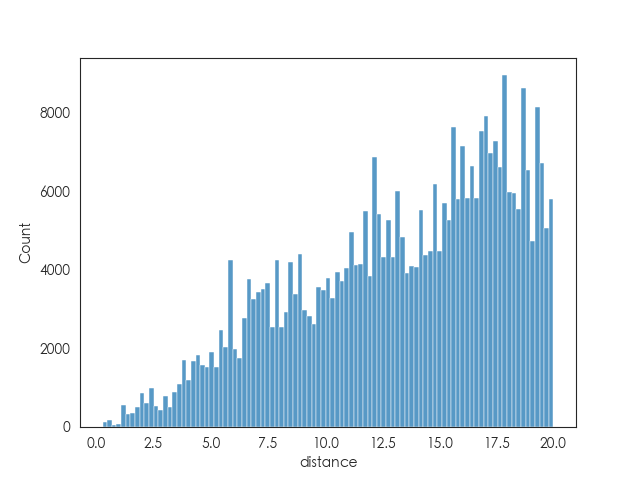
\includegraphics[width=\linewidth]{lib/img/olsdistance.png}
        \caption{标的与监测站距离分布}
    \end{minipage}
    \begin{minipage}{0.48\linewidth}
        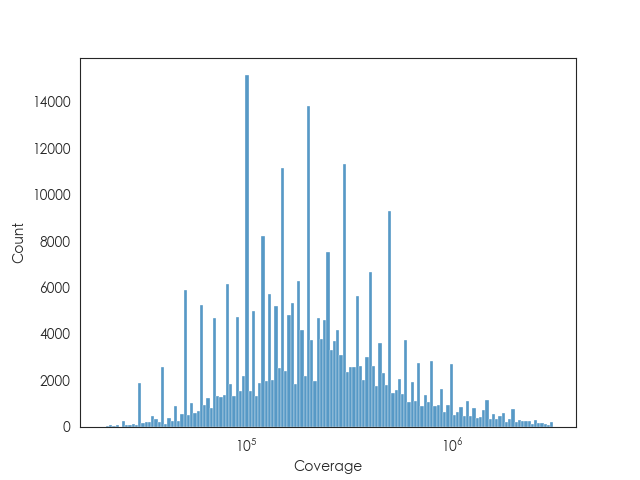
\includegraphics[width=\linewidth]{lib/img/coverage.png}
        \caption{标的保额对数分布}
    \end{minipage}
\end{figure}
\begin{figure}[H]
    \begin{minipage}{0.48\linewidth}
        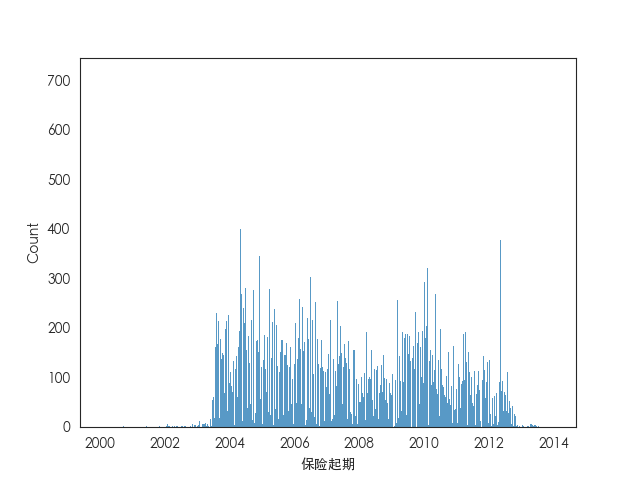
\includegraphics[width=\linewidth]{img/insurance.png}
        \caption{保险标的保险起期分布}
    \end{minipage}
    \begin{minipage}{0.48\linewidth}
        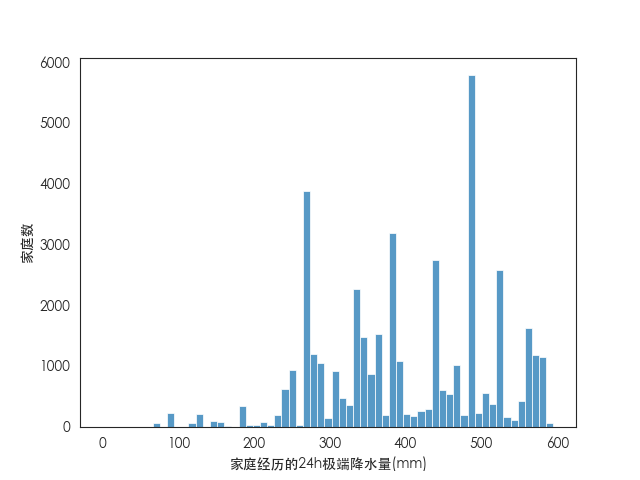
\includegraphics[width=\linewidth]{lib/img/precip.png}
        \caption{灾区家庭经历极端降水量的对数分布}
        TODO:对齐图,用没取对数的
    \end{minipage}
\end{figure}
% 截止2012年7月22日凌晨2时,北京全市平均降雨量164毫米,城区平均降雨量212毫米,降雨最大点在房山区河北镇,降雨量519毫米。
% \begin{table}[H]
%     \caption{变量之间相关性}\label{tab:corr}
%     \centering
%     \begin{tabular}{lrrrrrrr}
\toprule
 & Coverage & Disaster & Neighbor & Post & Prem\_before & Price & Area \\
\midrule
Coverage & 1.000000 & -0.003438 & 0.002232 & 0.006549 & 0.049063 & 0.195955 & -0.000131 \\
Disaster & -0.003438 & 1.000000 & -0.112619 & -0.199710 & -0.031179 & -0.027510 & -0.000619 \\
Neighbor & 0.002232 & -0.112619 & 1.000000 & -0.025723 & 0.004791 & 0.002799 & -0.000466 \\
Post & 0.006549 & -0.199710 & -0.025723 & 1.000000 & 0.014869 & 0.023873 & 0.000746 \\
Prem\_before & 0.049063 & -0.031179 & 0.004791 & 0.014869 & 1.000000 & 0.080722 & -0.000330 \\
Price & 0.195955 & -0.027510 & 0.002799 & 0.023873 & 0.080722 & 1.000000 & -0.000173 \\
Area & -0.000131 & -0.000619 & -0.000466 & 0.000746 & -0.000330 & -0.000173 & 1.000000 \\
\bottomrule
\end{tabular}


% \end{table}

\section{基准回归结果}
% \subsection{模型\ref{eq:OLS}:基础回归}
% 对于假设\ref{hyp:1},回归结果见表\ref{tab:ols}。

% \begin{table}[htbp]
%     \centering
%     \caption{OLS回归结果}\label{tab:ols}
%     
\begin{tabular}{@{\extracolsep{5pt}}lcc}
\\[-1.8ex]\hline
\hline \\[-1.8ex]
& \multicolumn{2}{c}{\textit{Dependent variable: log(Coverage)}} \
\cr \cline{2-3}
\\[-1.8ex] & (1) & (2) \\
\hline \\[-1.8ex]
 Area & & -0.000$^{}$ \\
& & (0.000) \\
 Intercept & 12.265$^{***}$ & 12.158$^{***}$ \\
& (0.004) & (0.003) \\
 Post & 0.100$^{***}$ & 0.071$^{***}$ \\
& (0.004) & (0.004) \\
 Prem\_before & & 0.670$^{***}$ \\
& & (0.008) \\
 Price & & 0.136$^{***}$ \\
& & (0.001) \\
\hline \\[-1.8ex]
 Observations & 414961 & 414961 \\
 $R^2$ & 0.001 & 0.171 \\
 Adjusted $R^2$ & 0.001 & 0.171 \\
 Residual Std. Error & 1.021 (df=414959) & 0.930 (df=414956) \\
 F Statistic & 584.020$^{***}$ (df=1; 414959) & 21392.415$^{***}$ (df=4; 414956) \\
\hline
\hline \\[-1.8ex]
\textit{Note:} & \multicolumn{2}{r}{$^{*}$p$<$0.1; $^{**}$p$<$0.05; $^{***}$p$<$0.01} \\
\end{tabular}

% \end{table}

\subsection{近灾区的DID回归}
对于假设\ref{hyp:3},回归结果见表\ref{tab:did1}。回归结果显示,在控制了其他变量之后,近灾区的交互项$\text{Neighbor}\times \text{Post}$的系数显著为正,这一结果验证了假设\ref{hyp:3},意味着在极端天气事件发生后,近灾区的保额提升了约23\%。近灾区居民由于接收到更丰富的信息,对极端天气事件的敏感度增强,因此他们的保险需求也相应增加。这种信息的丰富性可能来自于更直接的灾害经历、媒体报道、社区讨论等多种渠道,使得近灾区居民对灾害的潜在影响有了更深刻的认识。
\begin{table}[H]
    \centering
    \caption{实验组为近灾区的DID回归结果}\label{tab:did1}
    
\begin{tabular}{@{\extracolsep{5pt}}lcc}
\\[-1.8ex]\hline
\hline \\[-1.8ex]
& \multicolumn{2}{c}{\textit{Dependent variable: log(Coverage)}} \
\cr \cline{2-3}
\\[-1.8ex] & (1) & (2) \\
\hline \\[-1.8ex]
 Area & & -0.000$^{}$ \\
& & (0.000) \\
 Intercept & 12.164$^{***}$ & 12.067$^{***}$ \\
& (0.005) & (0.004) \\
 Neighbor & 0.227$^{***}$ & 0.224$^{***}$ \\
& (0.013) & (0.012) \\
 Neighbor:Post & 0.086$^{***}$ & 0.087$^{***}$ \\
& (0.015) & (0.014) \\
 Post & 0.095$^{***}$ & 0.068$^{***}$ \\
& (0.005) & (0.005) \\
 Prem\_before & & 0.542$^{***}$ \\
& & (0.008) \\
 Price & & 0.153$^{***}$ \\
& & (0.001) \\
\hline \\[-1.8ex]
 Observations & 455107 & 455107 \\
 $R^2$ & 0.006 & 0.136 \\
 Adjusted $R^2$ & 0.006 & 0.136 \\
 Residual Std. Error & 1.150 (df=455103) & 1.072 (df=455100) \\
 F Statistic & 961.465$^{***}$ (df=3; 455103) & 11948.789$^{***}$ (df=6; 455100) \\
\hline
\hline \\[-1.8ex]
\textit{Note:} & \multicolumn{2}{r}{$^{*}$p$<$0.1; $^{**}$p$<$0.05; $^{***}$p$<$0.01} \\
\end{tabular}

\end{table}

此外,当极端天气事件发生(即$\text{Post=1}$)时,不论家庭是否是否位于近灾区,家财险的保额整体上提高了约10\%。这一提升是显著为正,意味着在极端天气事件的影响下,家庭的风险感知得到了加强,从而增加了他们对家财险的需求。这一发现与假设\ref{hyp:3}的预期一致,即极端天气事件通过提高风险感知,导致家财险需求的提升。

控制变量方面,回归结果还表明,在家庭层面,保险标的的购置价每提升1\%导致保额平均提升0.36\%,家庭之前投保过会导致保额平均提升24\%。这两个变量的系数显著为正,与直觉相符,即价值较高的财和有保险购买历史的家庭更倾向于购买更高额度的保险。而在地区层面,GDP增速每增加1\%,家财险的保额整体上小幅提高约0.001\%,反应经济发展水平对保险需求的正向提升作用\citep{JJYJ200401002,arena2008does};而保险深度每提升1\%,家财险的保额整体上提高约0.67\%,反应保险市场的发展对保险需求的正向提升作用\citep{JRYJ200706018}。这两个变量的系数显著为正,与保险需求与经济发展水平、保险市场发展水平正相关的理论预期一致。

% 此外,DID回归结果还揭示了近灾区与远灾区之间的差异。近灾区的系数显著为正,表明与远灾区相比,近灾区的居民在灾害发生后购买的家财险保额提升了约22\%。这一差异可能源于近灾区居民对极端降水概率的主观判断更高,因此他们的风险感知也更强。这种强烈的风险感知可能促使他们购买更高额度的保险,以更好地保护自己的财产。

\subsection{灾区的DID回归}
对于假设\ref{hyp:2},回归结果见表\ref{tab:did2}。与表\ref{tab:did1}类似,该组也验证了假设\ref{hyp:3},即极端天气事件发生后购买家财险的保额提升约10\%。但是,交互项$\text{Disaster}\times \text{Post}$的系数为负,即灾区相对非灾区在受灾后反而降低了14\%保额,完全抵消了受灾后的10\%保额增加的影响,保额反而相对降低。其他控制变量的结果与表\ref{tab:did2}基本一致,保险标的的购置价、家庭之前投保过、GDP增速、保险深度等变量的系数符号与表\ref{tab:did1}一致,且显著性水平也基本一致。

TODO: note
\begin{table}[H]
    \centering
    \caption{实验组为灾区的DID回归结果}\label{tab:did2}
    
\begin{tabular}{@{\extracolsep{5pt}}lcc}
\\[-1.8ex]\hline
\hline \\[-1.8ex]
& \multicolumn{2}{c}{\textit{Dependent variable: log(Coverage)}} \
\cr \cline{2-3}
\\[-1.8ex] & (1) & (2) \\
\hline \\[-1.8ex]
 Area & & -0.000$^{}$ \\
& & (0.000) \\
 Disaster & 0.187$^{***}$ & 0.207$^{***}$ \\
& (0.009) & (0.008) \\
 Disaster:Post & -0.333$^{***}$ & -0.310$^{***}$ \\
& (0.011) & (0.010) \\
 Intercept & 12.164$^{***}$ & 12.071$^{***}$ \\
& (0.005) & (0.005) \\
 Post & 0.095$^{***}$ & 0.069$^{***}$ \\
& (0.005) & (0.005) \\
 Prem\_before & & 0.547$^{***}$ \\
& & (0.008) \\
 Price & & 0.144$^{***}$ \\
& & (0.001) \\
\hline \\[-1.8ex]
 Observations & 480733 & 480733 \\
 $R^2$ & 0.002 & 0.116 \\
 Adjusted $R^2$ & 0.002 & 0.116 \\
 Residual Std. Error & 1.163 (df=480729) & 1.095 (df=480726) \\
 F Statistic & 360.218$^{***}$ (df=3; 480729) & 10506.506$^{***}$ (df=6; 480726) \\
\hline
\hline \\[-1.8ex]
\textit{Note:} & \multicolumn{2}{r}{$^{*}$p$<$0.1; $^{**}$p$<$0.05; $^{***}$p$<$0.01} \\
\end{tabular}

\end{table}

\section{稳健性检验}
\subsection{平行趋势检验}

为了验证DID实证结果的稳健性,需要进行平行趋势检验。表\ref{tab:robust}展示了平行趋势检验的结果,并可视化如图\ref{fig:robust}。本文分别将实验组设置为灾区和近灾区($\text{Treat}=\text{Disaster}$以及$\text{Treat}=\text{Neighbor}$),对极端天气事件发生前四个季度的保额进行回归。回归结果显示交互项的系数都不显著,这表明在极端天气事件发生前,实验组和对照组的保额水平基本是平行的,满足平行趋势假设,可以通过DID方法来估计极端天气事件对家财险需求的影响。
% 唯一表现出显著性的部分是在灾区受灾前90天内(一个季度)的保额,这可能是因为20年一遇的极端降水往往是持续较久的,灾区居民达到20年一遇的门槛前已经开始感知到风险,从而提前购买了保险。

\begin{figure}[H]
    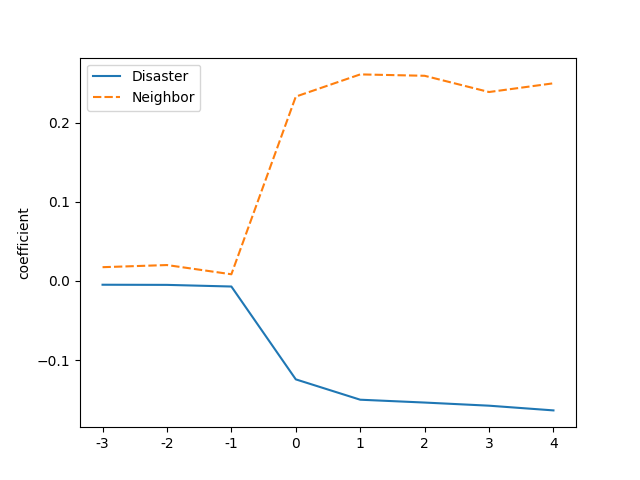
\includegraphics[width=\linewidth]{lib/img/robust.png}
    \caption{平行趋势检验}\label{fig:robust}
\end{figure}
\begin{table}[H]
    \centering
    \renewcommand{\arraystretch}{0.8}
    \caption{平行趋势检验}\label{tab:robust}
    
\begin{tabular}{@{\extracolsep{5pt}}lcc}
\\[-1.8ex]\hline
\hline \\[-1.8ex]
& \multicolumn{2}{c}{\textit{Dependent variable: log(Coverage)}} \
\cr \cline{2-3}
\\[-1.8ex] & \multicolumn{1}{c}{Disaster} & \multicolumn{1}{c}{Neighbor}  \\
\\[-1.8ex] & (1) & (2) \\
\hline \\[-1.8ex]
 Treated:C(Quarter)[T.-1] & -0.007$^{}$ & 0.008$^{}$ \\
& (0.015) & (0.042) \\
 Treated:C(Quarter)[T.-2] & -0.005$^{}$ & 0.020$^{}$ \\
& (0.015) & (0.040) \\
 Treated:C(Quarter)[T.-3] & -0.005$^{}$ & 0.017$^{}$ \\
& (0.014) & (0.041) \\
 Treated:C(Quarter)[T.0] & -0.124$^{***}$ & 0.233$^{***}$ \\
& (0.011) & (0.030) \\
 Treated:C(Quarter)[T.1] & -0.150$^{***}$ & 0.261$^{***}$ \\
& (0.013) & (0.030) \\
 Treated:C(Quarter)[T.2] & -0.153$^{***}$ & 0.259$^{***}$ \\
& (0.013) & (0.030) \\
 Treated:C(Quarter)[T.3] & -0.157$^{***}$ & 0.238$^{***}$ \\
& (0.013) & (0.030) \\
 Treated:C(Quarter)[T.4] & -0.163$^{***}$ & 0.250$^{***}$ \\
& (0.013) & (0.030) \\
C(Quarter)[T.-1] & -0.006$^{}$ & -0.006$^{}$ \\
& (0.009) & (0.009) \\
 C(Quarter)[T.-2] & -0.004$^{}$ & -0.004$^{}$ \\
& (0.009) & (0.009) \\
 C(Quarter)[T.-3] & -0.002$^{}$ & -0.002$^{}$ \\
& (0.009) & (0.009) \\
 C(Quarter)[T.0] & 0.091$^{***}$ & 0.095$^{***}$ \\
& (0.007) & (0.007) \\
 C(Quarter)[T.1] & 0.096$^{***}$ & 0.099$^{***}$ \\
& (0.007) & (0.007) \\
 C(Quarter)[T.2] & 0.097$^{***}$ & 0.101$^{***}$ \\
& (0.007) & (0.007) \\
 C(Quarter)[T.3] & 0.096$^{***}$ & 0.100$^{***}$ \\
& (0.007) & (0.007) \\
 C(Quarter)[T.4] & 0.101$^{***}$ & 0.105$^{***}$ \\
& (0.007) & (0.007) \\
 Treated & -0.002$^{}$ & -0.211$^{***}$ \\
& (0.010) & (0.029) \\
 Controls & True & True \\
 Intercept & 10.986$^{***}$ & 11.042$^{***}$ \\
& (0.007) & (0.007) \\
\hline \\[-1.8ex]
 Observations & 709271 & 654504 \\
 $R^2$ & 0.385 & 0.364 \\
 Adjusted $R^2$ & 0.385 & 0.364 \\
 Residual Std. Error & 0.661  & 0.677  \\
 F Statistic & 21157.483$^{***}$  & 17827.292$^{***}$  \\
\hline
\hline \\[-1.8ex]
\textit{Note:} & \multicolumn{2}{r}{$^{*}$p$<$0.1; $^{**}$p$<$0.05; $^{***}$p$<$0.01} \\
\end{tabular}

\end{table}

\subsection{安慰剂检验}
为排除其他潜在政策和遗漏变量等对回归结果的干扰,本文参考\citet{CYJJ202104009}随机虚构处理组,将 Neighbor 和 Disaster 的 DID 随机分组分配重复 500 次,结果如图\ref{fig:randomtest}所示。随机分配结果的所有系数估计值大体呈均值为 0 的正态分布,说明实验结果不是由于其他潜在政策或遗漏变量引起的,而是由于极端天气事件的影响。
\begin{figure}[H]
    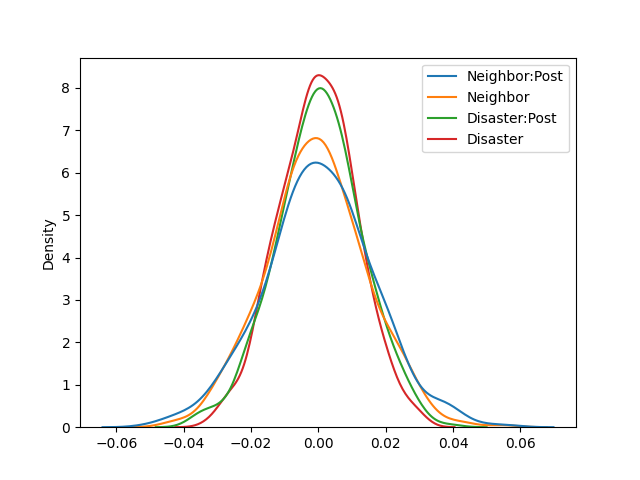
\includegraphics[width=\linewidth]{lib/img/randomtest.png}
    \caption{安慰剂检验}\label{fig:randomtest}
\end{figure}

\subsection{其他稳健性检验}

为保证基准回归结果的稳健性,本文还进行了以下稳健性检验:(1)(2)更换家财险需求的度量方式为保费Premium;(3)(4)/(5)(6)参考\citet{alok2020fund}分别将灾区距离上界从 20km 改为10km。回归结果如表\ref{tab:robustdid}所示。就回归结果而言,基本与基准回归结果一致,表明本文的实证结果是稳健的。这一结果进一步验证了极端天气事件通过增强家庭的风险感知,导致家财险需求的提升。
\begin{sidewaystable}[htbp]
    \centering
    \caption{稳健性检验回归结果}\label{tab:robustdid}
    
\begin{tabular}{@{\extracolsep{5pt}}lcccccc}
\\[-1.8ex]\hline
\hline \\[-1.8ex]
\\[-1.8ex] & \multicolumn{1}{c}{log(Premium)} & \multicolumn{1}{c}{log(Premium)} & \multicolumn{1}{c}{<30km} & \multicolumn{1}{c}{<30km} & \multicolumn{1}{c}{<10km} & \multicolumn{1}{c}{<10km}  \\
\\[-1.8ex] & (1) & (2) & (3) & (4) & (5) & (6) \\
\hline \\[-1.8ex]
 Area & 0.000$^{}$ & 0.000$^{}$ & 0.000$^{}$ & 0.000$^{}$ & 0.000$^{}$ & 0.000$^{}$ \\
& (0.000) & (0.000) & (0.000) & (0.000) & (0.000) & (0.000) \\
 Disaster & & -0.149$^{***}$ & & 0.187$^{***}$ & & 0.170$^{***}$ \\
& & (0.009) & & (0.006) & & (0.011) \\
 Disaster:Post & & -0.036$^{***}$ & & -0.207$^{***}$ & & -0.277$^{***}$ \\
& & (0.011) & & (0.007) & & (0.013) \\
 Intercept & 6.257$^{***}$ & 6.255$^{***}$ & 12.052$^{***}$ & 12.055$^{***}$ & 12.086$^{***}$ & 12.106$^{***}$ \\
& (0.005) & (0.005) & (0.003) & (0.003) & (0.006) & (0.006) \\
 Neighbor & 0.065$^{***}$ & & 0.222$^{***}$ & & 0.158$^{***}$ & \\
& (0.013) & & (0.012) & & (0.014) & \\
 Neighbor:Post & 0.024$^{}$ & & 0.150$^{***}$ & & 0.209$^{***}$ & \\
& (0.015) & & (0.013) & & (0.016) & \\
 Post & 0.097$^{***}$ & 0.097$^{***}$ & -0.000$^{}$ & -0.000$^{}$ & 0.085$^{***}$ & 0.098$^{***}$ \\
& (0.005) & (0.005) & (0.003) & (0.003) & (0.002) & (0.002) \\
 Prem\_before & -0.801$^{***}$ & -0.785$^{***}$ & 0.574$^{***}$ & 0.576$^{***}$ & 0.386$^{***}$ & 0.395$^{***}$ \\
& (0.009) & (0.009) & (0.006) & (0.006) & (0.009) & (0.010) \\
 Price & 0.084$^{***}$ & 0.086$^{***}$ & 0.184$^{***}$ & 0.178$^{***}$ & 0.238$^{***}$ & 0.198$^{***}$ \\
& (0.001) & (0.001) & (0.001) & (0.001) & (0.001) & (0.001) \\
\hline \\[-1.8ex]
 Observations & 408439 & 433025 & 853757 & 939148 & 270762 & 277046 \\
 $R^2$ & 0.041 & 0.038 & 0.150 & 0.131 & 0.190 & 0.146 \\
 Adjusted $R^2$ & 0.041 & 0.038 & 0.150 & 0.131 & 0.190 & 0.146 \\
 Residual Std. Error & 1.138  & 1.143  & 1.076  & 1.098  & 1.022  & 1.065  \\
 F Statistic & 2885.524$^{***}$  & 2880.383$^{***}$  & 25027.608$^{***}$  & 23637.295$^{***}$  & 10588.824$^{***}$  & 7863.860$^{***}$  \\
\hline
\hline \\[-1.8ex]
\textit{Note:} & \multicolumn{6}{r}{$^{*}$p$<$0.1; $^{**}$p$<$0.05; $^{***}$p$<$0.01} \\
\end{tabular}

\end{sidewaystable}

具体而言,表\ref{tab:robustdid}的模型(1)(2)显示,当极端天气事件发生后,家庭的保费整体上提高了约5\%。这一提升是显著为正,意味着在极端天气事件的影响下,家庭的风险感知得到了加强,从而增加了他们对家财险的需求。这一发现与假设\ref{hyp:3}的预期一致,即极端天气事件通过提高风险感知,导致家财险需求的提升。但灾区交互项的系数为负,表明灾区的保费在受灾后反而降低了约16\%,近灾区则提升了约57\%,与假设\ref{hyp:3}、假设\ref{hyp:2}一致。

就更改距离而言,模型(3)(4)/(5)(6)分别更改灾区受灾半径的上界至10km/30km,整体而言并不会改变实证结果,同样显示出灾区灾后保额购买减少约10-15\%、近灾区保额购买提升25-30\%,表明本文的实证结果是稳健的。

%!root = ../main.tex
\chapter{进一步的分析}\label{chap:4.1}
在基础回归的基础上,本文将在基准回归的基础上进行进一步的分析,主要探讨灾区平均保额在极端降水冲击后降低的可能原因。

在分析灾区平均保额在极端天气冲击后降低的现象时,本文提出冲击导致损失不足、低估冲击再次发生概率和新低保额保单摊薄三个可能的解释:

首先,降水冲击可能带来损失比较有限。从居民的心理预期角度来看,当灾区居民经历极端天气事件后,他们可能会重新评估灾害风险,发现实际的损失并没有达到预期的严重程度\citep{谢晓非2012心理台风眼效应研究综述,王大伟2014先前情绪和过度自信对灾难事件后继风险决策的影响},甚至没有达到免赔额。这种认知上的变化可能导致他们认为高额的保险投保并不必要,因此选择降低保险额度,以减少未来的保险费用支出。这种情况下,可以观察到灾区居民获得理赔概率相对于非灾区在灾后变化不大,因此居民保额需求减少。基于此本文定义是保单否理赔为$\text{Claimed}$,建立如下Logit DID回归模型:
\begin{equation}
    logit(\text{Claimed}_{it}) =\beta_0 +\beta_1 \text{Disaster}_i+\beta_2\text{Post}_{it}+\beta_3\text{Disaster}_i \times \text{Post}_{it} + Controls_{it}+ \varepsilon_{it}
    \label{eq:1}
\end{equation}

其次,居民可能低估极端降水冲击再次发生概率,“闪电不可能击中同一个地方两次”。居民可能认为,在极端降水冲击发生后,短期内再次发生极端降水冲击的概率较低\citep{szollosi2019simultaneous},因此平均保额有所下降,以减少不必要的保险费用。这种情况下,可以观察到居民续保的概率相对于非灾区在灾后变小,从而导致保险需求减少。基于此本文定义是保单否是否续保为$\text{Renew}$,建立如下Logit DID回归模型:
\begin{equation}
    logit(\text{Renew}_{it}) =\beta_0 +\beta_1 \text{Disaster}_i+\beta_2\text{Post}_{it}+\beta_3\text{Disaster}_i \times \text{Post}_{it} + Controls_{it}+ \varepsilon_{it}
    \label{eq:2}
\end{equation}

最后,平均保额的减少也可能是由于大量低保额的新保单加入。这种情况意味着灾区居民在受灾后风险感知增强,但新增的保险需求偏低,导致整体呈现出家财险平均保额减少。这种情况下,可以观察到灾区非续保保单的平均保额相对于灾区续保保单在灾后显著变小。基于此,本文定义非续保保单为$\text{First}$,针对灾区保单建立如下OLS DID回归模型:
\begin{equation}\label{eq:3}
    \log(\text{Coverage}_{it}) =\beta_0 + \beta_1 \text{First}_{it} + \beta_2 \text{Post}_{it}+\beta_3 \text{Post}_{it} \times \text{First}_{it} + Controls_{it}+ \varepsilon_{it}
\end{equation}

式(\ref{eq:1})、(\ref{eq:2})和(\ref{eq:3})的回归结果如表\ref{tab:renew}所示。从表中可以看出:
\begin{enumerate}
    \item 针对式(\ref{eq:1}),灾区居民在极端降水冲击后,$\text{Disaster}\times\text{Post}$显著为正,说明获得理赔概率相对于非灾区有所上升,说明保险起到了转移风险的作用。因此灾区冲击后平均保额下降原因并不是居民认为冲击后损失有限。
    \item 针对式(\ref{eq:2}),灾区居民在极端降水冲击后,$\text{Disaster}\times\text{Post}$显著为负,即灾后续保概率相对于非灾区显著下降,说明尽管降水冲击带来损失(式\ref{eq:1}),但居民认为短时间内再次发生极端降水冲击的概率较低,续保动力不足,平均保额下降。
    \item 针对式(\ref{eq:3}),$\text{First}$系数显著为负,灾区内首次投保的保单在冲击发生前平均保额就低于续保保单,与表\ref{tab:did1}与\ref{tab:did2}中非首次投保保额更高一致。但是交互项$\text{First}\times\text{Post}$系数并不显著,说明降水冲击对于首次投保保单的影响较小。
\end{enumerate}

\begin{table}[ht]
    \caption{进一步分析回归结果}\label{tab:renew}
    \centering
    
\begin{tabular}{@{\extracolsep{5pt}}lcccc}
\\[-1.8ex]\hline
\hline \\[-1.8ex]
\\[-1.8ex] & \multicolumn{1}{c}{Claim} & \multicolumn{1}{c}{Claim} & \multicolumn{1}{c}{Renew} & \multicolumn{1}{c}{Renew}  \\
\\[-1.8ex] & (1) & (2) & (3) & (4) \\
\hline \\[-1.8ex]
 Disaster & 0.405$^{**}$ & 0.391$^{**}$ & -3.773$^{***}$ & -3.706$^{***}$ \\
& (0.169) & (0.169) & (0.221) & (0.222) \\
 Disaster:Post & 0.630$^{***}$ & 0.622$^{***}$ & 2.243$^{***}$ & 2.232$^{***}$ \\
& (0.190) & (0.190) & (0.234) & (0.235) \\
 Intercept & -6.825$^{***}$ & -4.664$^{***}$ & -5.228$^{***}$ & -11.891$^{***}$ \\
& (0.166) & (0.675) & (0.053) & (0.169) \\
 Post & -0.167$^{}$ & -0.158$^{}$ & -0.556$^{***}$ & -0.525$^{***}$ \\
& (0.123) & (0.123) & (0.028) & (0.029) \\
 Prem\_before & -2.299$^{***}$ & -2.246$^{***}$ & 4.428$^{***}$ & 4.338$^{***}$ \\
& (0.708) & (0.709) & (0.020) & (0.020) \\
 log(Coverage) & & -0.212$^{***}$ & & 0.668$^{***}$ \\
& & (0.067) & & (0.015) \\
 log(GDP) & -0.001$^{}$ & -0.001$^{}$ & 0.013$^{***}$ & 0.013$^{***}$ \\
& (0.006) & (0.006) & (0.002) & (0.002) \\
 log(Penetration) & -0.645$^{***}$ & -0.551$^{***}$ & 2.541$^{***}$ & 2.448$^{***}$ \\
& (0.152) & (0.156) & (0.056) & (0.056) \\
 log(Price) & 0.013$^{}$ & 0.140$^{**}$ & 0.499$^{***}$ & 0.031$^{***}$ \\
& (0.030) & (0.061) & (0.011) & (0.010) \\
\hline \\[-1.8ex]
 Observations & 709271 & 709271 & 709271 & 709271 \\
 Pseudo $R^2$ & 0.012 & 0.013 & 0.368 & 0.377 \\
 Yera FE & True & True & True & True \\
\hline
\hline \\[-1.8ex]
\textit{Note:} & \multicolumn{4}{r}{$^{*}$p$<$0.1; $^{**}$p$<$0.05; $^{***}$p$<$0.01} \\
\end{tabular}

\end{table}
\chapter{结论与建议}\label{chap:5}

\section{研究结论}

本研究通过对极端降水冲击的准自然实验,探讨了极端天气事件对家财险需求的影响。基于某保险公司的家财险数据,采用差分分析方法,我们得出了以下主要结论:
\begin{enumerate}
    \item 极端天气事件显著提高了居民的风险感知,尤其是对于近灾区的居民。这种风险感知的提升促使居民更加关注家庭财产的保护,从而增加了对家财险的需求,近灾区居民在极端天气事件冲击后保额需求提升约24\%。这表明在面对气候变化带来的风险时,公众的保险意识有所增强。

    \item 但与此同时,对于直接受到极端天气事件冲击的地区,家财险需求并未显著增加,反而可能减少约18\%。这背后可能是由于家庭认为短期内再次遭受巨灾的概率不大,因而在受灾后对家财险需求减少。

    \item 不同地区居民对极端天气事件的反应存在一定差异。东部和中部地区居民在遭受极端降水事件后,保险金额有所下降,而在近灾区,保险金额的增长更为显著。而西部地区灾区居民对极端降水事件的反应则与东部和中部地区有所不同,保额会在灾后显著提升。这可能是由于西部地区居民对极端降水风险的敏感度在灾前较低,灾后意识到了风险导致保险需求增加的幅度较大。

    \item 2008年金融危机和汶川地震事件对家庭风险感知产生了显著影响,正向提升了家庭在灾后的保险需求。这表明家庭在感知到巨大风险后,对保险的需求可能会有所增加。

    \item 家庭财产的价值对保险需求也产生了影响。保险标的价值越高,近灾区的保险需求增加越明显,而灾区的保险需求则可能降低更明显。这可能是由于近灾区家庭对高价值家庭财产的损失更为敏感,而灾区家庭则可能认为短期内不会再次受灾,因此保险需求减少。

    \item 地级市与县区居民对极端天气事件的反应也存在差异。县区居民对极端天气事件的风险感知程度更高,保险需求增加的幅度相对较大。这可能是由于县区居民与农业联系更紧密,对极端天气事件的风险感知程度更高,但与此同时保险覆盖率相对较低,因此在灾后保险需求增加的幅度相对较大。
\end{enumerate}
\section{政策建议}
\subsection{保险公司视角:创新产品与宣传,提高保障水平}
面对全球气候变化带来的挑战,极端天气事件的频发已成为不容忽视的现象。在这样的背景下,保险公司必须采取更加主动和创新的策略,帮助社会管理极端天气事件带来的风险,提高家庭的风险抵御能力。

首先,保险公司应深入洞察极端天气事件对不同地域、不同时间节点以及不同价值保险标的影响,以此为基础,创新和优化家财险产品。这意味着保险公司需开发出更具针对性的保险产品,满足不同客户群体在面临气候变化风险时的多样化需求。例如,对于高风险区域,可以设计更高覆盖范围的保险产品;对于价值较高的家财,可以提供更高保额的保险选项。

其次,保险公司需加强风险评估与定价策略的研究,确保保险费率既能合理反映风险水平,又能为受灾家庭提供足够的保障。这需要保险公司运用先进的风险管理技术和数据分析方法,精准评估极端天气事件带来的潜在风险。

再次,保险公司应加强宣传教育工作,提高公众对极端天气事件风险的认识,以及保险在风险管理中的作用。通过教育和宣传,保险公司可以帮助公众更好地理解保险产品的价值,从而提高保险意识,增强家庭的抗风险能力。

最后,保险公司应与政府、科研机构以及其他相关部门密切合作,共同研究气候变化的新趋势,以及这些变化对保险需求的潜在影响。通过跨部门合作,保险公司不仅可以获得更多的数据和研究成果支持,还可以在政策制定中发挥积极作用,为构建更加安全、可持续的社会贡献力量。

保险公司作为社会风险管理的重要一环,其在应对极端天气事件中的作为与担当,不仅关乎企业的发展,更关乎社会的稳定与人民的福祉。愿保险公司能以此研究为契机,不断进取,为推动保险行业的健康发展,为社会的和谐与进步作出更大的贡献。

\subsection{政府视角:对保障不足的潜在灾区提供补贴}
政府在应对应急管理中扮演着至关重要的角色。在深刻认识到极端天气事件对家财险需求影响的基础上,政府应采取一系列措施,提高家庭的风险抵御能力,保障公众的生命财产安全。

首先,政府应加强对极端天气事件的监测与预警系统的建设,提升公众的风险意识。通过建立健全的灾害预警机制,政府可以确保在极端天气事件发生前,及时向公众发布预警信息,引导居民采取必要的防范措施,减少灾害带来的损失。

其次,政府应考虑为潜在灾区的居民提供保险补贴,尤其是对于经济较为落后的地区。通过财政补贴等手段,政府可以降低家庭购买家财险的经济负担,提高保险覆盖率,增强家庭的抗风险能力。

再次,政府应鼓励和支持保险公司开发与推广针对极端天气事件的保险产品。在政策上给予一定的倾斜和优惠,如税收减免、资金扶持等,激发保险公司的创新活力,满足市场对此类保险产品的需求。

此外,政府应加强与保险公司的合作,共同开展气候变化风险管理的宣传教育活动。通过提高公众对气候变化和极端天气事件的认识,增强社会的风险防范意识,促进保险文化的普及。

最后,政府应制定相应的政策,鼓励和引导保险公司参与到国家的防灾减灾工作中来。保险公司作为风险管理的专业机构,在灾害风险评估、风险转移等方面具有独特优势。政府可以通过公私合作模式,充分利用保险公司的资源和专长,提高国家防灾减灾的整体能力。

\appendix
\nocite{*}
\newrefcontext[sorting=nyt]
\printbibliography[heading = bibintoc, title = {参考文献}]
% %!TEX root = ../thesis.tex
% Copyright (c) 2014,2016 Casper Ti. Vector
% Public domain.

\chapter{附件}

% vim:ts=4:sw=4

\backmatter
\ifblind\else%!TEX root = ../thesis.tex
\chapter{致谢}

\fi
%!TEX root = ../thesis.tex
% Copyright (c) 2008-2009 solvethis
% Copyright (c) 2010-2017,2021 Casper Ti. Vector
% Copyright (c) 2021 Kurapica
% All rights reserved.
%
% Redistribution and use in source and binary forms, with or without
% modification, are permitted provided that the following conditions are
% met:
%
% * Redistributions of source code must retain the above copyright notice,
%   this list of conditions and the following disclaimer.
% * Redistributions in binary form must reproduce the above copyright
%   notice, this list of conditions and the following disclaimer in the
%   documentation and/or other materials provided with the distribution.
% * Neither the name of Peking University nor the names of its contributors
%   may be used to endorse or promote products derived from this software
%   without specific prior written permission.
%
% THIS SOFTWARE IS PROVIDED BY THE COPYRIGHT HOLDERS AND CONTRIBUTORS "AS
% IS" AND ANY EXPRESS OR IMPLIED WARRANTIES, INCLUDING, BUT NOT LIMITED TO,
% THE IMPLIED WARRANTIES OF MERCHANTABILITY AND FITNESS FOR A PARTICULAR
% PURPOSE ARE DISCLAIMED. IN NO EVENT SHALL THE COPYRIGHT HOLDER OR
% CONTRIBUTORS BE LIABLE FOR ANY DIRECT, INDIRECT, INCIDENTAL, SPECIAL,
% EXEMPLARY, OR CONSEQUENTIAL DAMAGES (INCLUDING, BUT NOT LIMITED TO,
% PROCUREMENT OF SUBSTITUTE GOODS OR SERVICES; LOSS OF USE, DATA, OR
% PROFITS; OR BUSINESS INTERRUPTION) HOWEVER CAUSED AND ON ANY THEORY OF
% LIABILITY, WHETHER IN CONTRACT, STRICT LIABILITY, OR TORT (INCLUDING
% NEGLIGENCE OR OTHERWISE) ARISING IN ANY WAY OUT OF THE USE OF THIS
% SOFTWARE, EVEN IF ADVISED OF THE POSSIBILITY OF SUCH DAMAGE.

{
	\ctexset{section = {
		format+ = {\centering}, beforeskip = {40bp}, afterskip = {15bp}
	}}
	\specialchap{北京大学学位论文原创性声明和使用授权说明}

	% 学校书面要求本页面不要页码,但在给出的 Word 模版中又有页码。
	% 此处以学校书面要求为准。
	\thispagestyle{empty}
	\mbox{}\vspace*{-3em}
	\section*{原创性声明}

	本人郑重声明:
	所呈交的学位论文,是本人在导师的指导下,独立进行研究工作所取得的成果。
	除文中已经注明引用的内容外,
	本论文不含任何其他个人或集体已经发表或撰写过的作品或成果。
	对本文的研究做出重要贡献的个人和集体,均已在文中以明确方式标明。
	本声明的法律结果由本人承担。
	\vskip 1em
	\rightline{%
		论文作者签名:\hspace{5em}%
		日期:\hspace{2em}年\hspace{2em}月\hspace{2em}日%
	}

	\section*{%
		学位论文使用授权说明\\[-0.33em]
		\textmd{\zihao{5}(必须装订在提交学校图书馆的印刷本)}%
	}

	本人完全了解北京大学关于收集、保存、使用学位论文的规定,即:
	\begin{itemize}
		\item 按照学校要求提交学位论文的印刷本和电子版本;
		\item 学校有权保存学位论文的印刷本和电子版,
			并提供目录检索与阅览服务,在校园网上提供服务;
		\item 学校可以采用影印、缩印、数字化或其它复制手段保存论文;
		\item 因某种特殊原因须要延迟发布学位论文电子版,
			授权学校 $\Box$\nobreakspace{}一年 /
			$\Box$\nobreakspace{}两年 /
			$\Box$\nobreakspace{}三年以后,在校园网上全文发布。
	\end{itemize}
	\centerline{(保密论文在解密后遵守此规定)}
	\vskip 1em
	\rightline{%
		论文作者签名:\hspace{5em}导师签名:\hspace{5em}%
		日期:\hspace{2em}年\hspace{2em}月\hspace{2em}日%
	}

	% 若须排版二维码,请将二维码图片重命名为“barcode”,
	% 转为合适的图片格式,并放在当前目录下,然后去掉下面 2 行的注释。
	\vfill\noindent
	
\includegraphics[height = 5em]{img/barcode.png}
}

% vim:ts=4:sw=4

\end{document}
%